\chapter{Implementation} \label{cap:implementation}

\section{Parallelization Strategy}

The parallelization strategy adopted for the Coin Counter is a divide-and-conquer approach implemented using the Fork/Join pattern with a \texttt{ForkJoinPool} and \texttt{RecursiveTask}. This pattern is particularly well-suited to the problem, as it efficiently parallelizes the recursive binary tree of calls generated by the sequential algorithm, which inherently explores two branches (including or excluding each coin) at every recursive step. It is a good solution because it matches the natural recursive structure of the sequential algorithm.

\section{Benchmark Results}

The benchmark results demonstrate a significant performance improvement when using the parallel implementation compared to the sequential version. As shown in Figure \ref{fig:benchmark_comparison}, the parallel approach enables processing larger coin sets in substantially shorter time frames.

\begin{figure}[H]
    \centering
    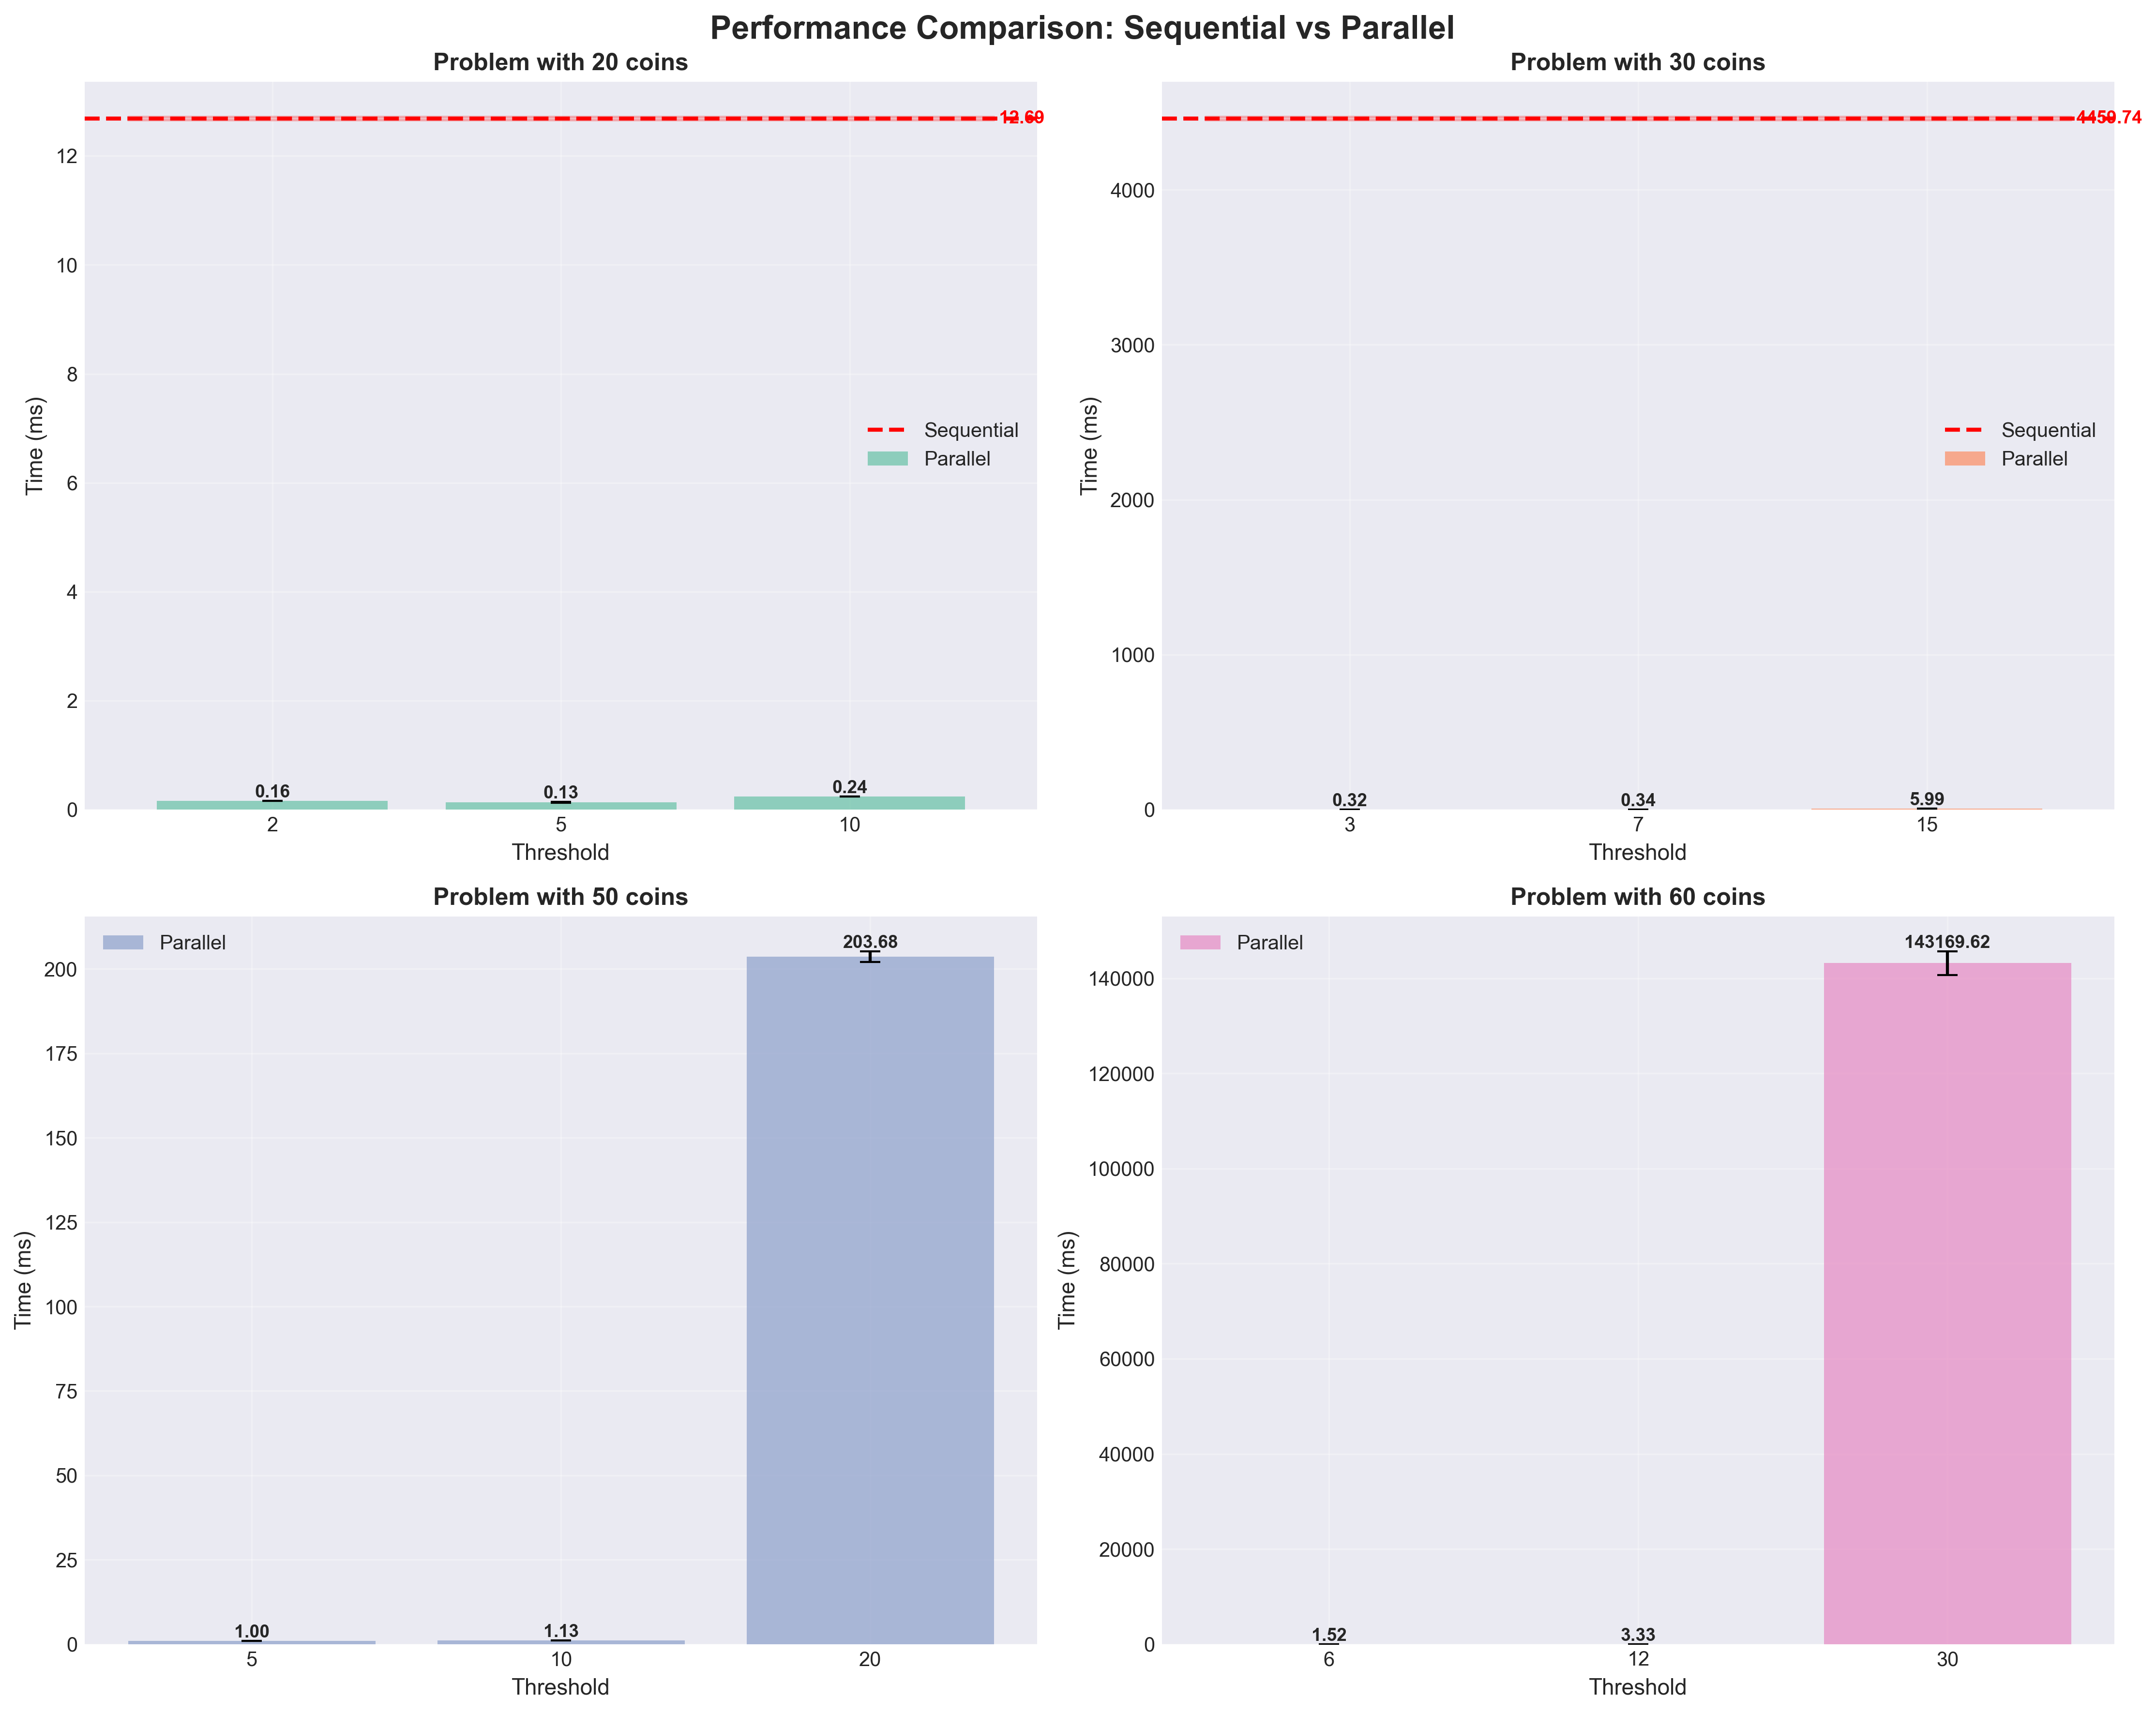
\includegraphics[width=0.8\textwidth]{images/benchmark_comparison.png}
    \caption{Performance comparison between Sequential and Parallel implementations across different problem sizes and threshold values.}
    \label{fig:benchmark_comparison}
\end{figure}

For the 20-coin problem, the parallel version achieves a speedup between 52.9x to 97.6x. Similarly, for 30 coins, it achieves speedups ranging from 744.53x to 13,936x.

The sequential version becomes impractical for problems larger than 30 coins due to its exponential time complexity. In contrast, the parallel implementation successfully handles 50 and 60 coins within reasonable time frames.

The threshold parameter has a crucial role in performance optimization. Lower threshold values (2-7 for smaller problems, 5-12 for larger ones) generally yield better performance. However, for the largest problem size (60 coins), a threshold of 30 results in significantly worse performance, suggesting that excessively fine-grained parallelization introduces overhead that outweighs its benefits.

These results confirm that the parallel implementation not only provides substantial speedups for problems solvable by the sequential version but also extends the practical range of solvable problem sizes, making it achievable to handle the coin problem with up to 60 coins that would be otherwise computationally impossible with a sequential approach.

\section{Improvements}

Beyond the parallelization improvements achieved through the Fork-Join pattern, the parallel implementation adds memoization to optimize performance. When a subproblem is encountered that has already been solved by another thread, its result is retrieved from a \texttt{ConcurrentHashMap} that uses a concatenated key of \texttt{(index, accumulator)} to uniquely identify each subproblem state. This memoization strategy dramatically reduces redundant calculations, particularly when multiple threads converge on identical subproblems during exploration of the solution space.
